

%\begin{figure}[ht]
%    \centering
%    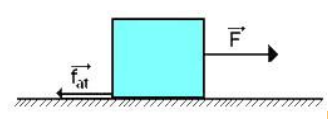
\includegraphics{JoseGeraldo-lista1/fig/fig1.png}
%    \caption{bloco com atrito}
%    
%    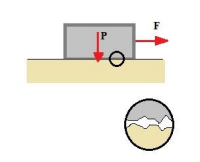
\includegraphics{JoseGeraldo-lista1/fig/fig2.png}
%    \caption{Rugosidades}
%\end{figure}


%\textbf{} //negrito 
%\begin{equation}
%            F_{a_t} = µ_e \times N
%            \label{equ:Atrito estatico}
%\end{equation}

%\section{Polias e Roldanas}
\section{Implementação do Gerador Congruencial Linear}
O código a seguir após implementado consegue receber um vetor por parâmetro e preenche-lo com valores gerados congruencialmente.
por parâmetro também são informados os seguintes dados:

\textbf{m: } modulo;

\textbf{a: } multiplicador;

\textbf{b: } incremento;

\textbf{noOfRandomNums: } quantidade de valores aleatórios.

\begin{figure}[ht]
    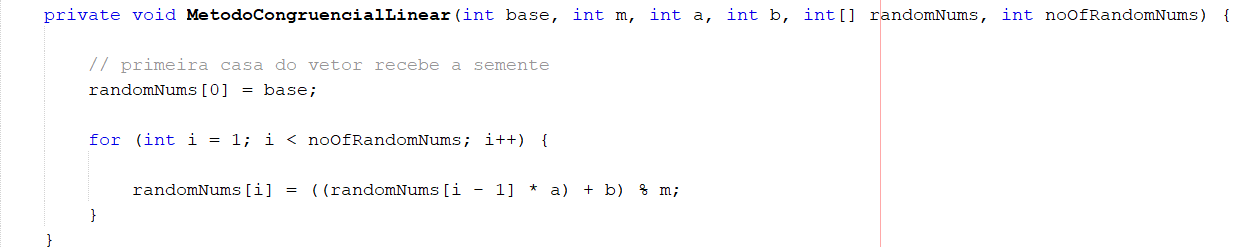
\includegraphics[scale=0.54]{JoseGeraldo-lista2/fig/fig2.png}
    \caption{Gerador Congruencial linear em Java \cite{site1}}
\end{figure}

Dado um número inicial conhecido como semente, o próximo número da sequência é dado pela seguinte equação:

\begin{equation}
            randomNums[0] = ((base * a) + b) \ \% \ m
            \label{equ: equação congruencial linear}
\end{equation}


Os valores sucessores são determinados pela seguinte equação:

\begin{equation}
            randomNums[i] = ((randomNums[i - 1] * a) + b) \ \% \ m
            \label{equ: equação congruencial linear}
\end{equation}

O operador \% indica resto da divisão. Os números assim gerados estão entre 0 e m-1 \cite{site3}.

Para a amostragem deste trabalho foram utilizados os seguintes valores:
\textbf{m: } 100000;

\textbf{a: } 157;

\textbf{b: } 1;

\textbf{noOfRandomNums: } 5000.

Com tais valores o código implementado gera um vetor de n posições preenchido com os valores resultantes do gerador.

\section{Estudo do Período}
Durante os teste do gerador é possível notar uma periodicidade nos valores gerados, onde de acordo com os valores pre definidos no mesmo é gerado um numero limitado de valores que se repetem após determinado período.

Para os valores informados na seção 2.1, foi possível obter os seguintes dados para este gerador:

\begin{figure}[ht]
    \centering
    
\includegraphics{JoseGeraldo-lista2/fig/fig3.png}
    \caption{Analise de período do gerador}

\end{figure}

Utilizando estes valores é possível plotar gráficos que ilustrem um padrão no processo de gerar números, comprovando que estes valores não são aleatórios.
A seguir serão apresentados 6 diferentes gráficos, que apresentam diferentes porcentagens do período do gerador implementado, quanto mais valores do período são utilizados para gerar coordenadas X e Y, mais visível o padrão se torna mais visível.

Para tal experimentação, os valores do período foram armazenados em um vetor, onde os valores armazenados neste vetor que possuem índice par representarão as coordenadas X, e os de índices impares as coordenadas Y.
\newpage
\begin{figure}[ht]

    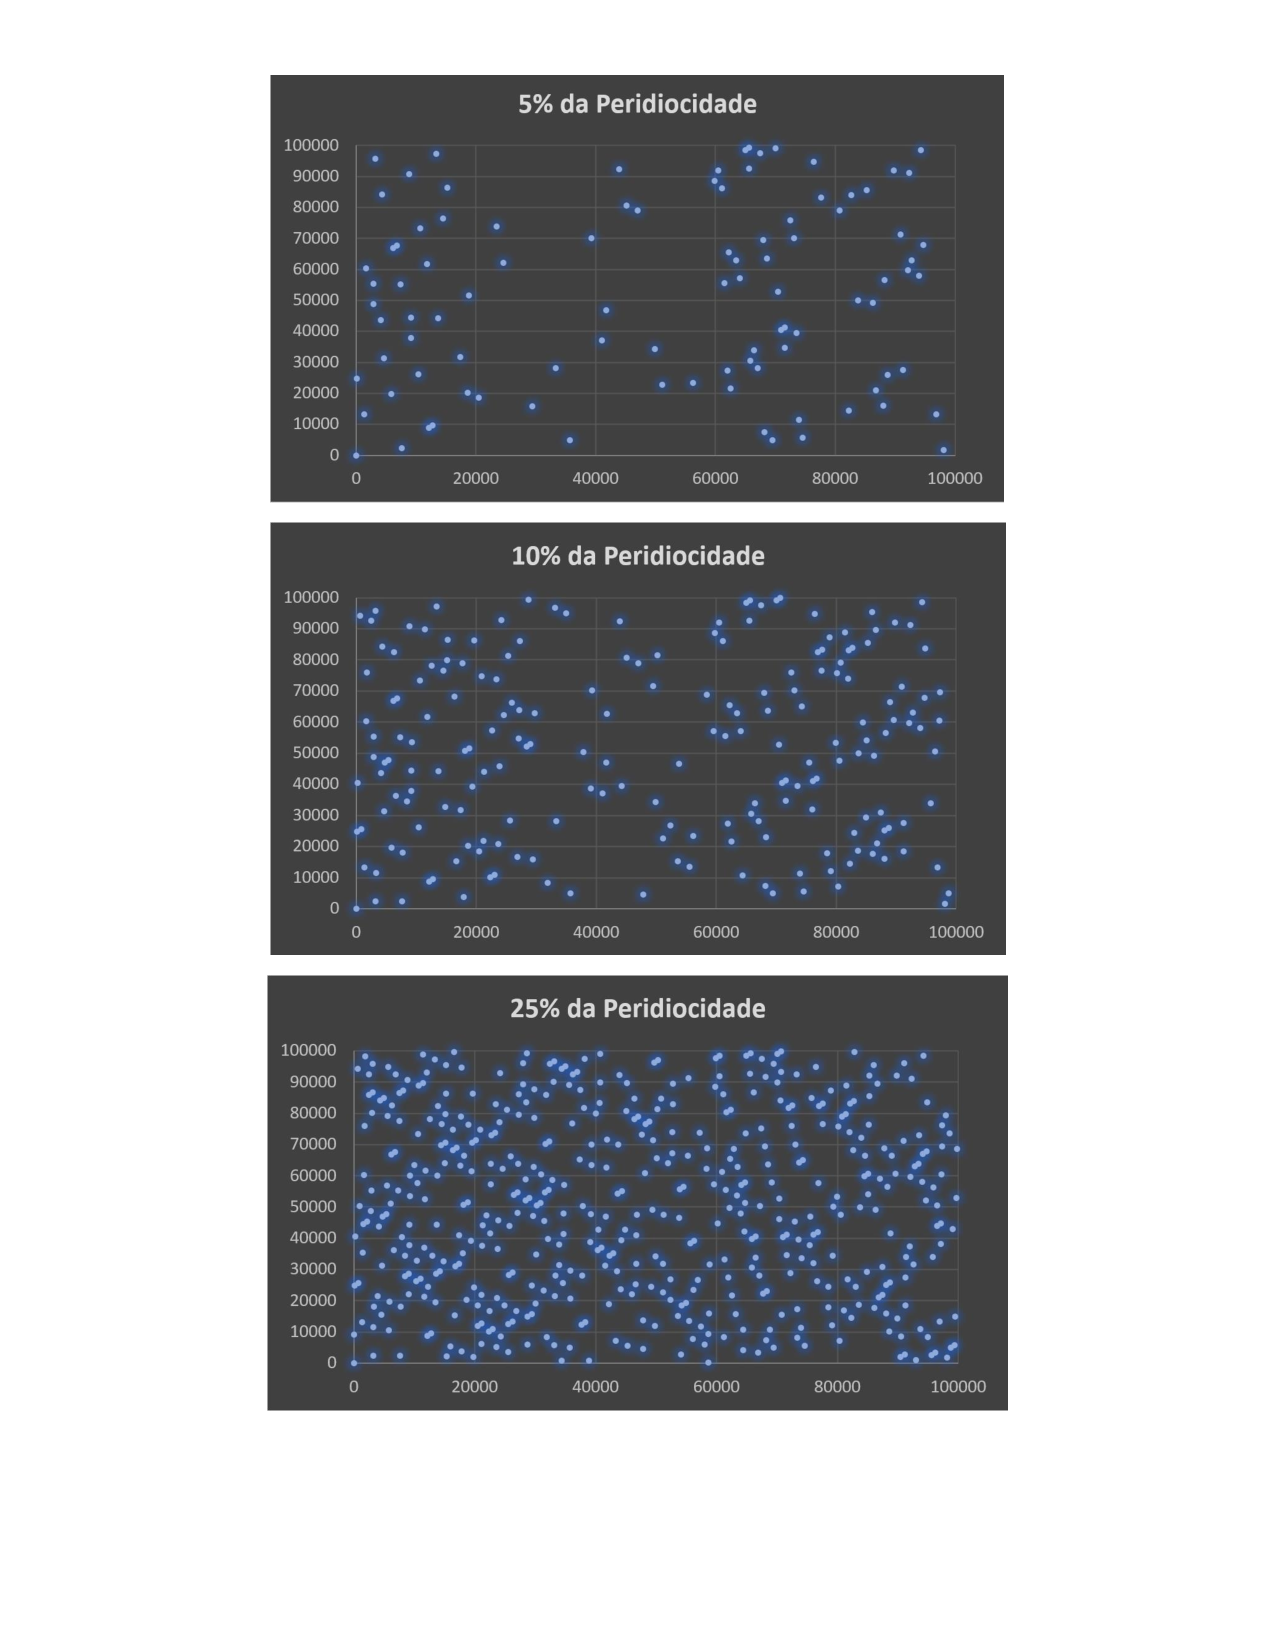
\includegraphics[scale=0.74]{JoseGeraldo-lista2/fig/fig1.pdf}
    \caption{Gráficos Períodos do Gerador (5\% a 25\%)}

\end{figure}
\newpage
\begin{figure}[ht]
    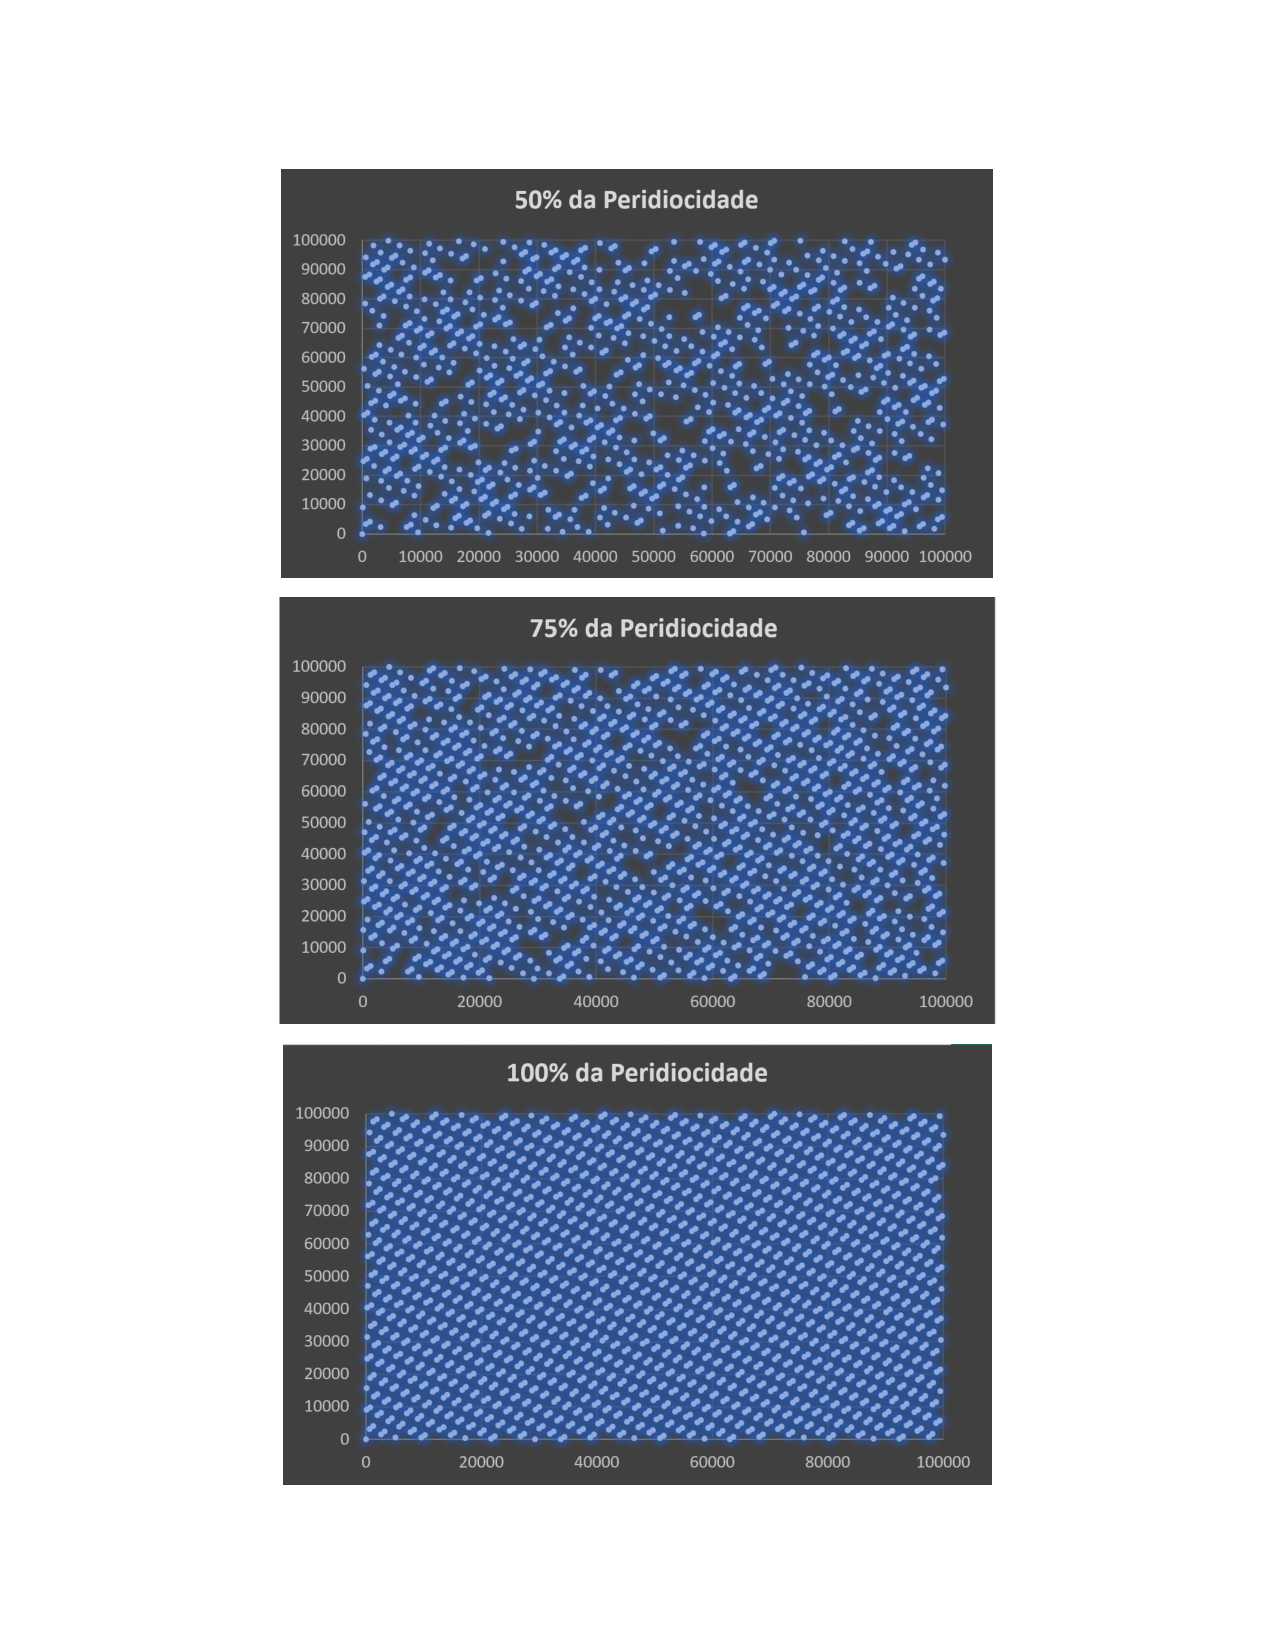
\includegraphics[scale=0.74]{JoseGeraldo-lista2/fig/fig4.pdf}
    \caption{Gráficos Períodos do Gerador - (50\% a 100\%)}

\end{figure}

\newpage
\section{Math.random}
Também é possível gerar números pseudoaleatórios usando o método estático random() da classe Math. Este método retorna um valor double no intervalo de 0.0 até 1.0, sem incluir este último valor (0.0 <= x < 1.0). Caso se necessite de outros intervalos de valores, será preciso efetuar operações aritméticas com os valores gerados, como por exemplo uma multiplicação\cite{site2}.

Um dado importante sobre o método Math.random é que ele, internamente, utiliza a própria classe java.util.Random para gerar os números aleatórios.
Para gerar números inteiros com esse método é necessário realizar cast para int do valor gerado\cite{site2}.

Para exemplificar a capacidade de gerar valores da biblioteca nativa do Java, foram gerados 4000 valores aleatórios, que foram posicionados em pares ordenados utilizando a mesma regra implementada nos testes do gerador congruencial.

Com estes teste foi possível ver que a amplitude entre a semente e o fim do periodo do gerador desta biblioteca é muito grande, onde nos teste não foi possivel ter uma percepção visual da pseudoaletoriedade.

Os resultados foram plotados no gráfico a seguir:

\begin{figure}[ht]
    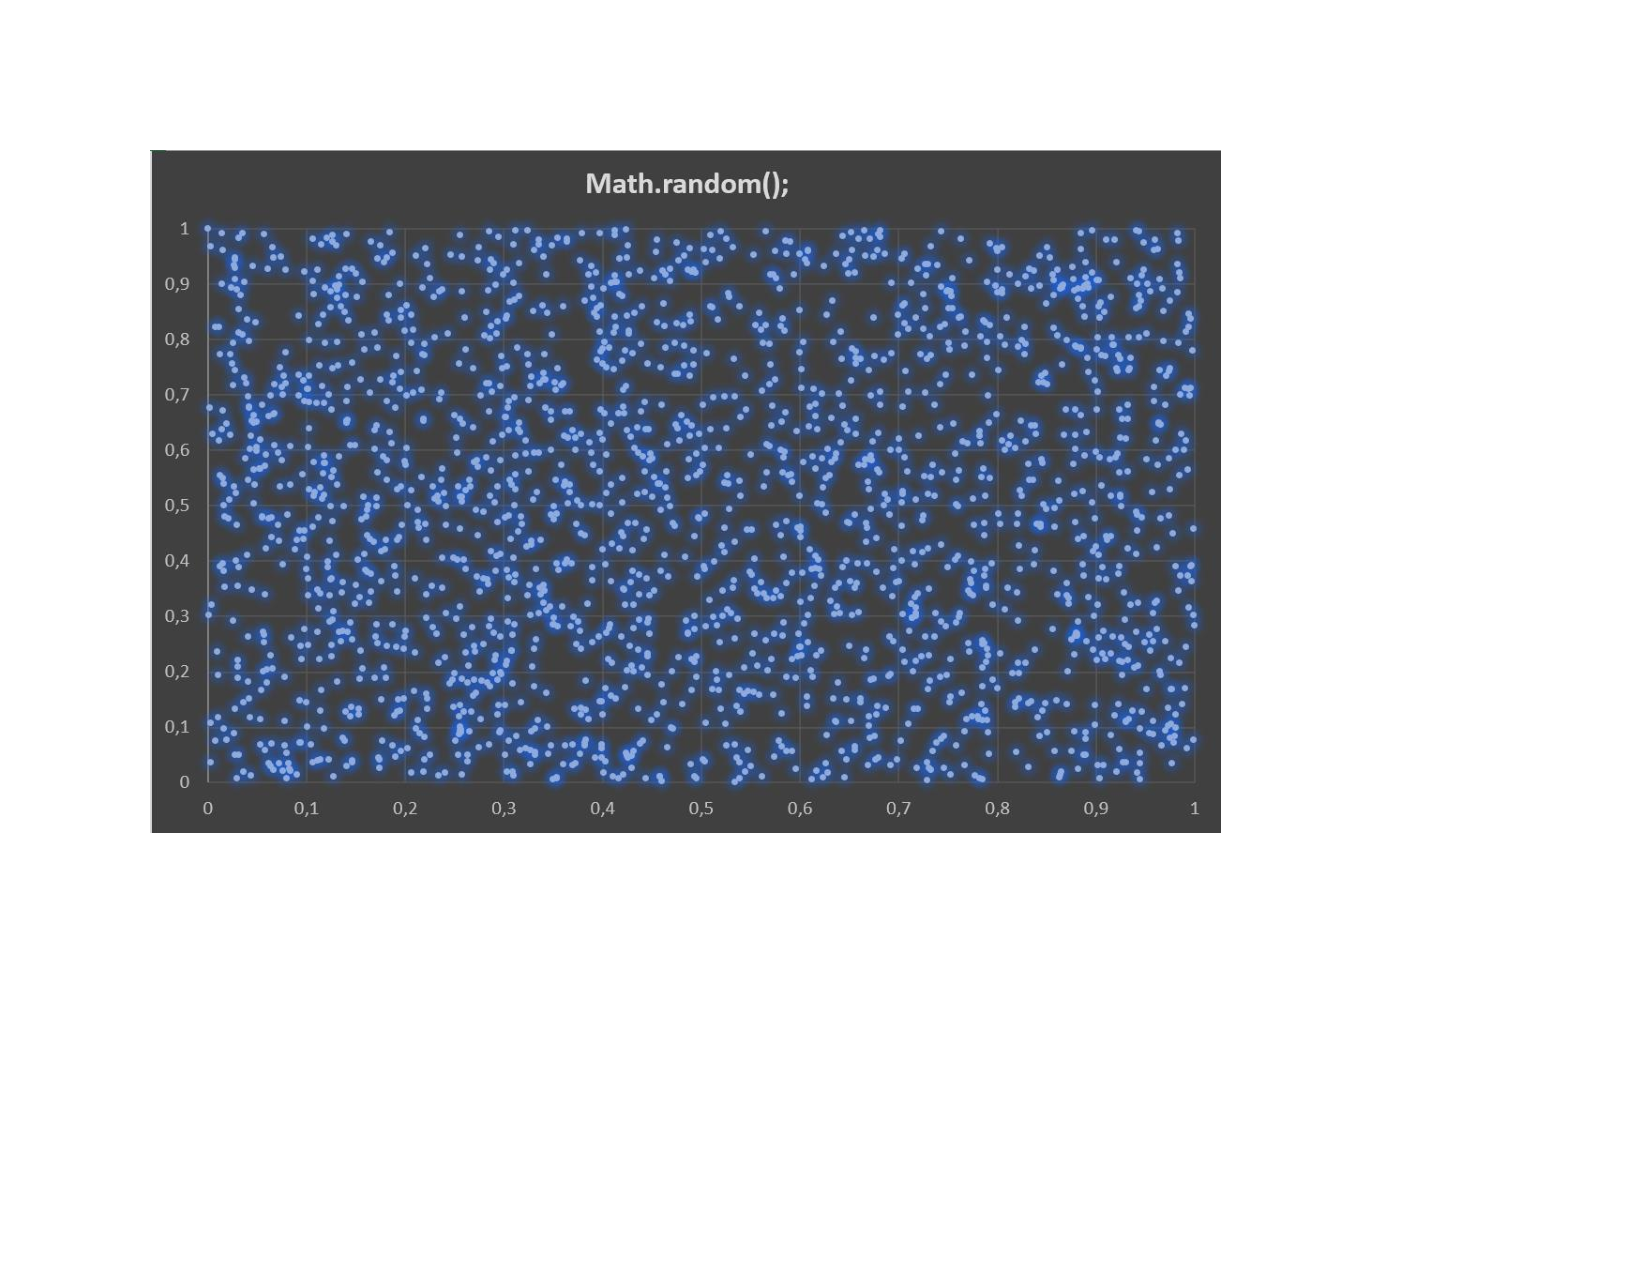
\includegraphics[scale=0.73]{JoseGeraldo-lista2/fig/fig5.pdf}
    \caption{Periodo de 2000 valores gerados na biblioteca Math.random()}

\end{figure}

